\section{Validierung}

- Fragen/Anforderungen vom Anfang erfüllt?\\

- Funktionsweise gegeben?\\
- Gpio Test mit Schaltung\\
- Spi Kommunitkation. Test mit Oszi (Screenshots)\\


Die Validierung der entwickelten Hardware-Abstraktionsschicht (HW\_API) dient dem Nachweis ihrer Funktionalität, Korrektheit und Plattformunabhängigkeit. 
Ziel dieser Untersuchung ist es, sicherzustellen, dass die implementierten Klassen sowohl auf STM32- als auch auf ESP32-Plattformen zuverlässig arbeiten und den gestellten Anforderungen entsprechen.
Die Überprüfung der Funktionalität wurden mehreren Schritten gewährleistet.
So musste zunächst bestätigt werden, dass der Code fehlerfrei kompiliert und gebaut wird.
Beim Debuggen musste festgestellt werden, ob das Programm sich so verhält, wie es erwartet ist oder ob unerwünschte Seiteneffekte auftreten.

\subsection{Testaufbau}
Um die korrekte Funktionsweise der Gpio-Klasse zu gewährleisten wurde mit einem Breadboard eine Schaltung mit einem Taster und einer LED aufgebaut.
Diese konnte dann die verfügbaren \gls{mcu}s an den konfigurierten Pins angeschlossen werden.

%\begin{figure}[H]
%	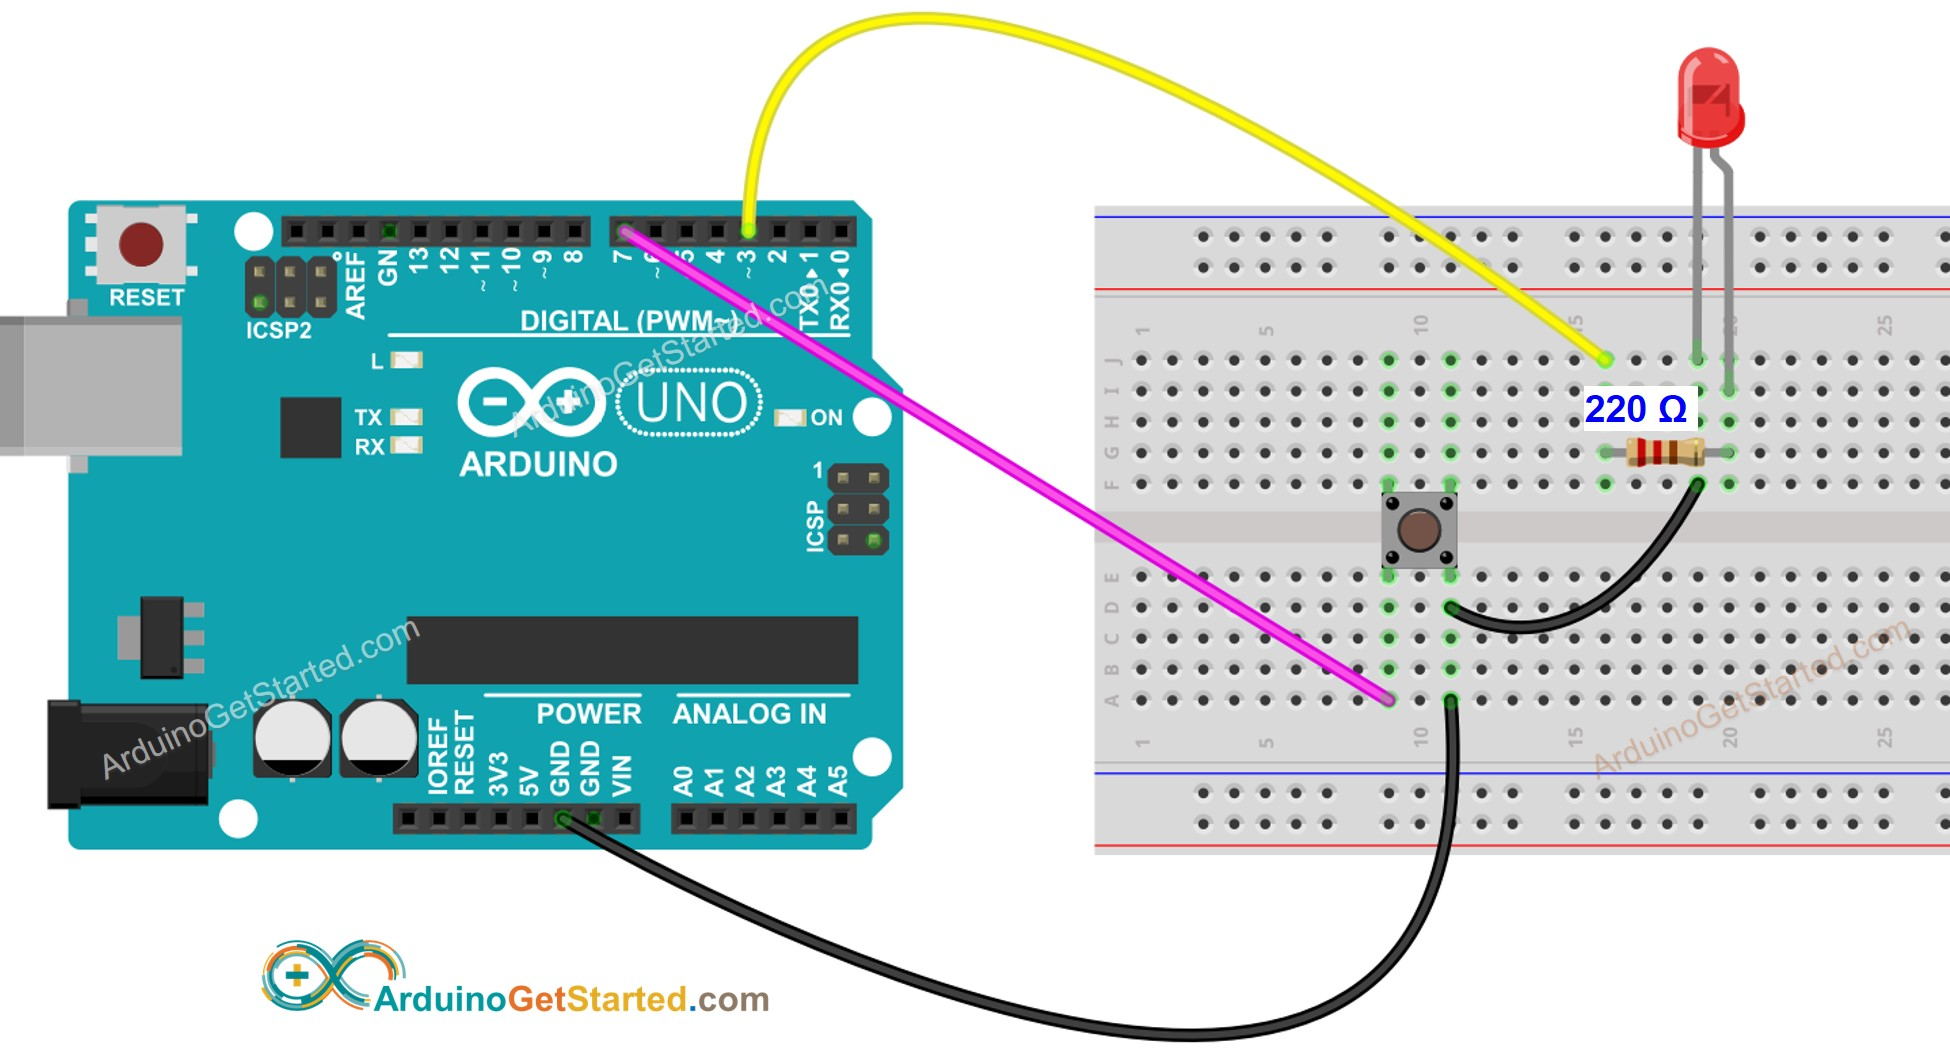
\includegraphics[width=\textwidth]{Pics/button-led-wiring-diagram.jpg}
%	\caption{Aufbau der Testschaltung, dargestellt durch ein Arduino-Hardware und einem Breadboard mit LED, einem 202 \Omega Widerstand und einem Taster.}
%	\label{fig:breadboard_wirinig}
%\end{figure}

Um die Funktionsweise der SPI- und DMA-Klassen zu überprüfen wurden ein Codeabschnitte implementiert: einer für einen Master, einer für einen Slave.
Die Pinkonfiguration war für beide die Gleiche.
Für jede Hardware wurde jeweils ein SPI-Objekt und ein DMA-Objekt erstellt.

Im Code wurde implementiert, dass der Master ein 'A' sendet und auf eine Antwort wartet, während der Slave ein 'O' sendet und eine Nachricht wartet.
Der Master-Code wurde auf ein STM32Nucleo-C031C6, der Slave-Code auf ein STM32Nucleo-G0B1RE geflasht. 
Die beiden MCUs wurden über die in der projct\_config.hpp definierte Gpio-Objekte mit einander verbunden.
An die einzelnen Pins wurden dann Klammern eines Oszilloskops angeschlossen um die Signale von Systemclock SCK, Master-Out-Slave-In MOSI, Master-In-Slave-Out MISO und NSS/CS Negative-Slave-Select bzw. Chip-Select zu beobachten. 

\subsection{Testergebnisse}
% CMakeLists, Build, Compile
Beginnend mit der Auswahl der Hardware durch die Kombination von Makefilekonfigurationen (stm32\_config.mk bzw. esp\_config.mk), CMakeLists-Struktur und Factory-Imlpementierung konnte Schritt für Schritt eine Struktur erarbeitet werden, die im weiteren Verlauf fehlerfrei funktioniert hat.
Bei unerwartetem Verhalten aber entsprechende Fehlermeldungen ausgeben konnte.
Im Fall von STM32 Hardware, da hiervon mehr zur Auswahl stand und diese auch hauptsächlich in der Praxis verwendet wird, hat auch der Wechsel zwischen unterschiedlichen Familien, STM32C0xx und STM32G0xx, über die stm32\_config.mk reibungslos funktioniert.
Der Einsatz von definierten Makros, wie beispielsweise \texttt{TARGET\_PLATFORM} \texttt{MCU\_FAMILY} oder \texttt{MCU\_SPECIFIC}, um in den CMakeLists.txt-Dateien die entsprechenden Bibliotheken auszuwählen, Dateien hinzuzufügen sowie Abschnitte freizuschalten, hat sich als vorteilhaft für die Erstellung eines automatisierten Kompilations- und Buildprozesses innerhalb der gesamten Struktur erwiesen.
Darüber hinaus hatte dies eine erfolgreiche Erstellung der Hardwareobjekte durch die Factory zur Folge.
Die wählt anhand der Makros erst die richtige Plattform und im weiteren Verlauf die spezifische Hardware aus.
% GPIO

Mit einem erstellten Programm, das die neuen Gpio-Objekte und deren Funktionen verwendet, und der aufgebauten Schaltung konnten das Lese und Schreib verhalten erfolgreich überprüft werden.
Bei Betätigung des Tasters sollte die LED eingeschaltet werden; bei erneuter Betätigung dementsprechend wieder ausgeschaltet werden.
Dieses Verhalten wurde erfolgreich umgesetzt.

% SPI
Um die
% Oszi-Bild , wie es aussehen sollte
\begin{figure}[H]
	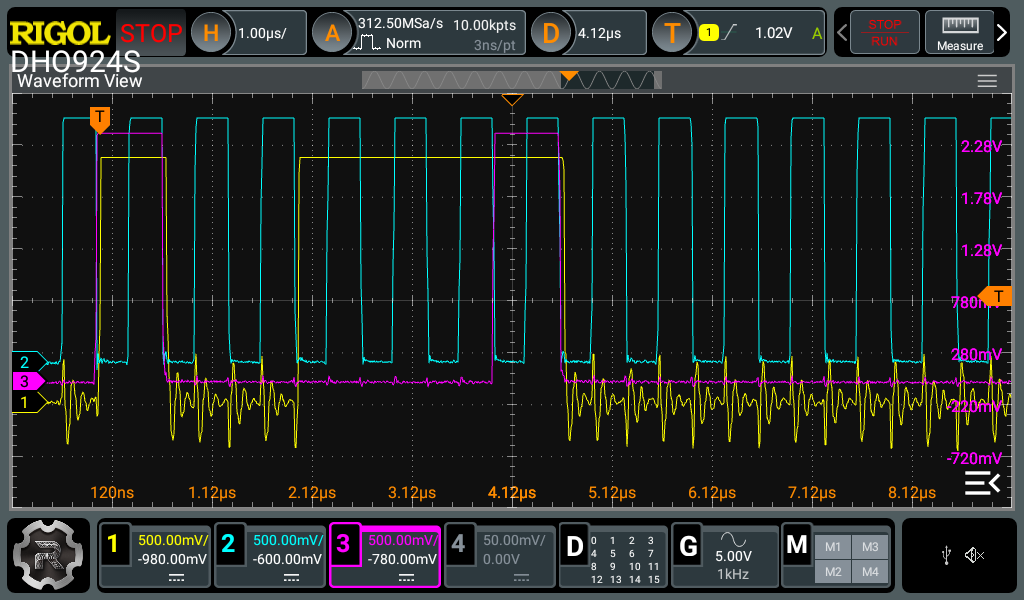
\includegraphics[width=\textwidth]{Pics/oszi_cube_spi_example.png}
	\caption{Screenshot des Osziloskopbildschirms. Dieser zeigt die Wellen für SCK (blau), MOSI (magenta) und MISO (gelb).}
	\label{fig:oszi_cube_spi_example}
\end{figure}

So sollten die Wellen auch mit dem Plattformunabhängigen Code aussehen.

\begin{figure}[H]
	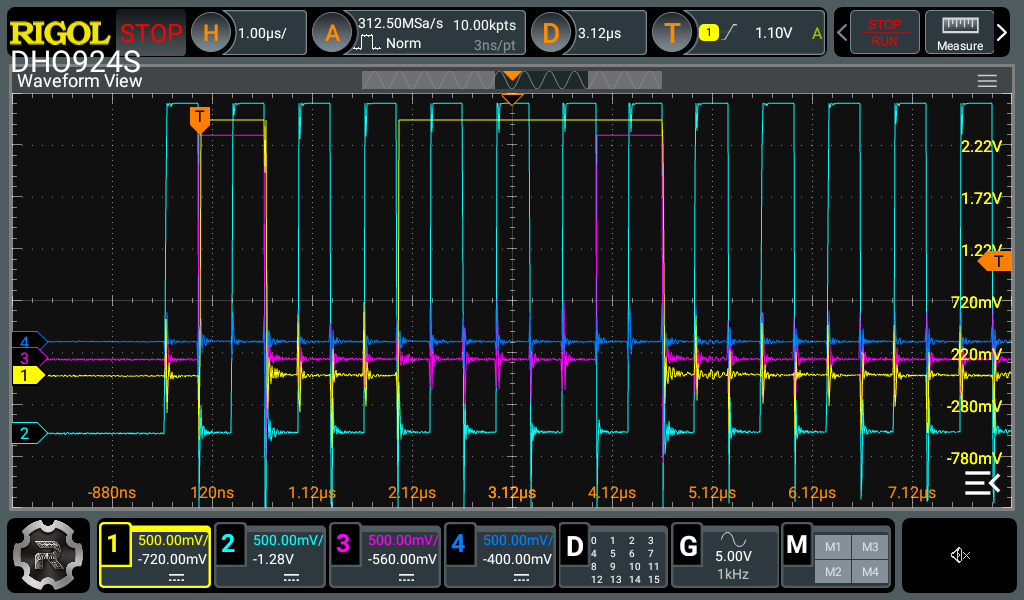
\includegraphics[width=\textwidth]{Pics/spi_signal_test.png}
	\caption{Screenshot einer erfolgreich SPI-Kommunikation, erstellt mit dem Code der HW\_API.}
\end{figure}


%Die Testumgebung umfasste sowohl das STM32C0-Board als auch ein ESP32-DevKit, jeweils verbunden mit Debug-Schnittstellen und notwendiger Peripherie.
%Die Tests wurden systematisch durchgeführt, indem jeder GPIO-Pin und jedes Peripheriemodul einzeln initialisiert, konfiguriert und gemessen wurde. 
%Für die SPI-Schnittstelle wurden verschiedene Kommunikationsszenarien simuliert, um mögliche Timing- oder Konfigurationsfehler zu erkennen.
%
%Die erzielten Ergebnisse zeigen, dass die HW\_API die spezifizierten Funktionen korrekt bereitstellt. 
%GPIO-Pins verhielten sich entsprechend der konfigurierten Pull-Up/Pull-Down-Einstellungen, und die SPI-Kommunikation konnte zuverlässig Daten übertragen. 
%Alle gemessenen Signalpegel lagen innerhalb der spezifizierten Grenzwerte der jeweiligen Plattformen. 
%Auffälligkeiten traten nicht auf, und die statische Analyse ergab keine kritischen Warnungen oder Verstöße gegen etablierte Embedded-Coding-Standards.
%
%Die Interpretation dieser Ergebnisse bestätigt die Robustheit und Portabilität der entwickelten Abstraktionsschicht. 
%Die modulare Struktur, die plattformspezifische Implementierungen sauber kapselt, erlaubt den Einsatz auf mehreren Mikrocontrollerfamilien, ohne dass Änderungen am Anwendungscode erforderlich sind. 
%Einschränkungen bestehen lediglich in der begrenzten Testabdeckung anderer STM32-Familien, die nicht direkt validiert wurden.

Zusammenfassend zeigt die Validierung, dass die HW\_API die geforderten funktionalen Anforderungen erfüllt, korrekt arbeitet und eine stabile Grundlage für die Implementierung plattformunabhängiger Embedded-Anwendungen darstellt. 
Die gewählten Testmethoden gewährleisten eine nachvollziehbare und reproduzierbare Überprüfung der Softwarequalität.











































